\documentclass[tikz,border=5pt]{standalone}
\usetikzlibrary{arrows.meta,backgrounds,calc,positioning}

\definecolor{processblue}{HTML}{A7D8D0}
\definecolor{atmosgreen}{HTML}{347A71}
\definecolor{meteopastel}{HTML}{76C7D8}
\definecolor{fertpastel}{HTML}{F2A675}
\definecolor{organicpastel}{HTML}{A8D5A2}
\definecolor{inputblue}{HTML}{006FE6}
\definecolor{outputpurple}{HTML}{9226D3}
\definecolor{nitratepink}{HTML}{F3B6C6}
\definecolor{nitrateborder}{HTML}{C96A85}
\definecolor{factorochre}{HTML}{A96F00}
\definecolor{factorfill}{HTML}{F4D58A}
\definecolor{textgray}{HTML}{2F2F2F}

\begin{document}
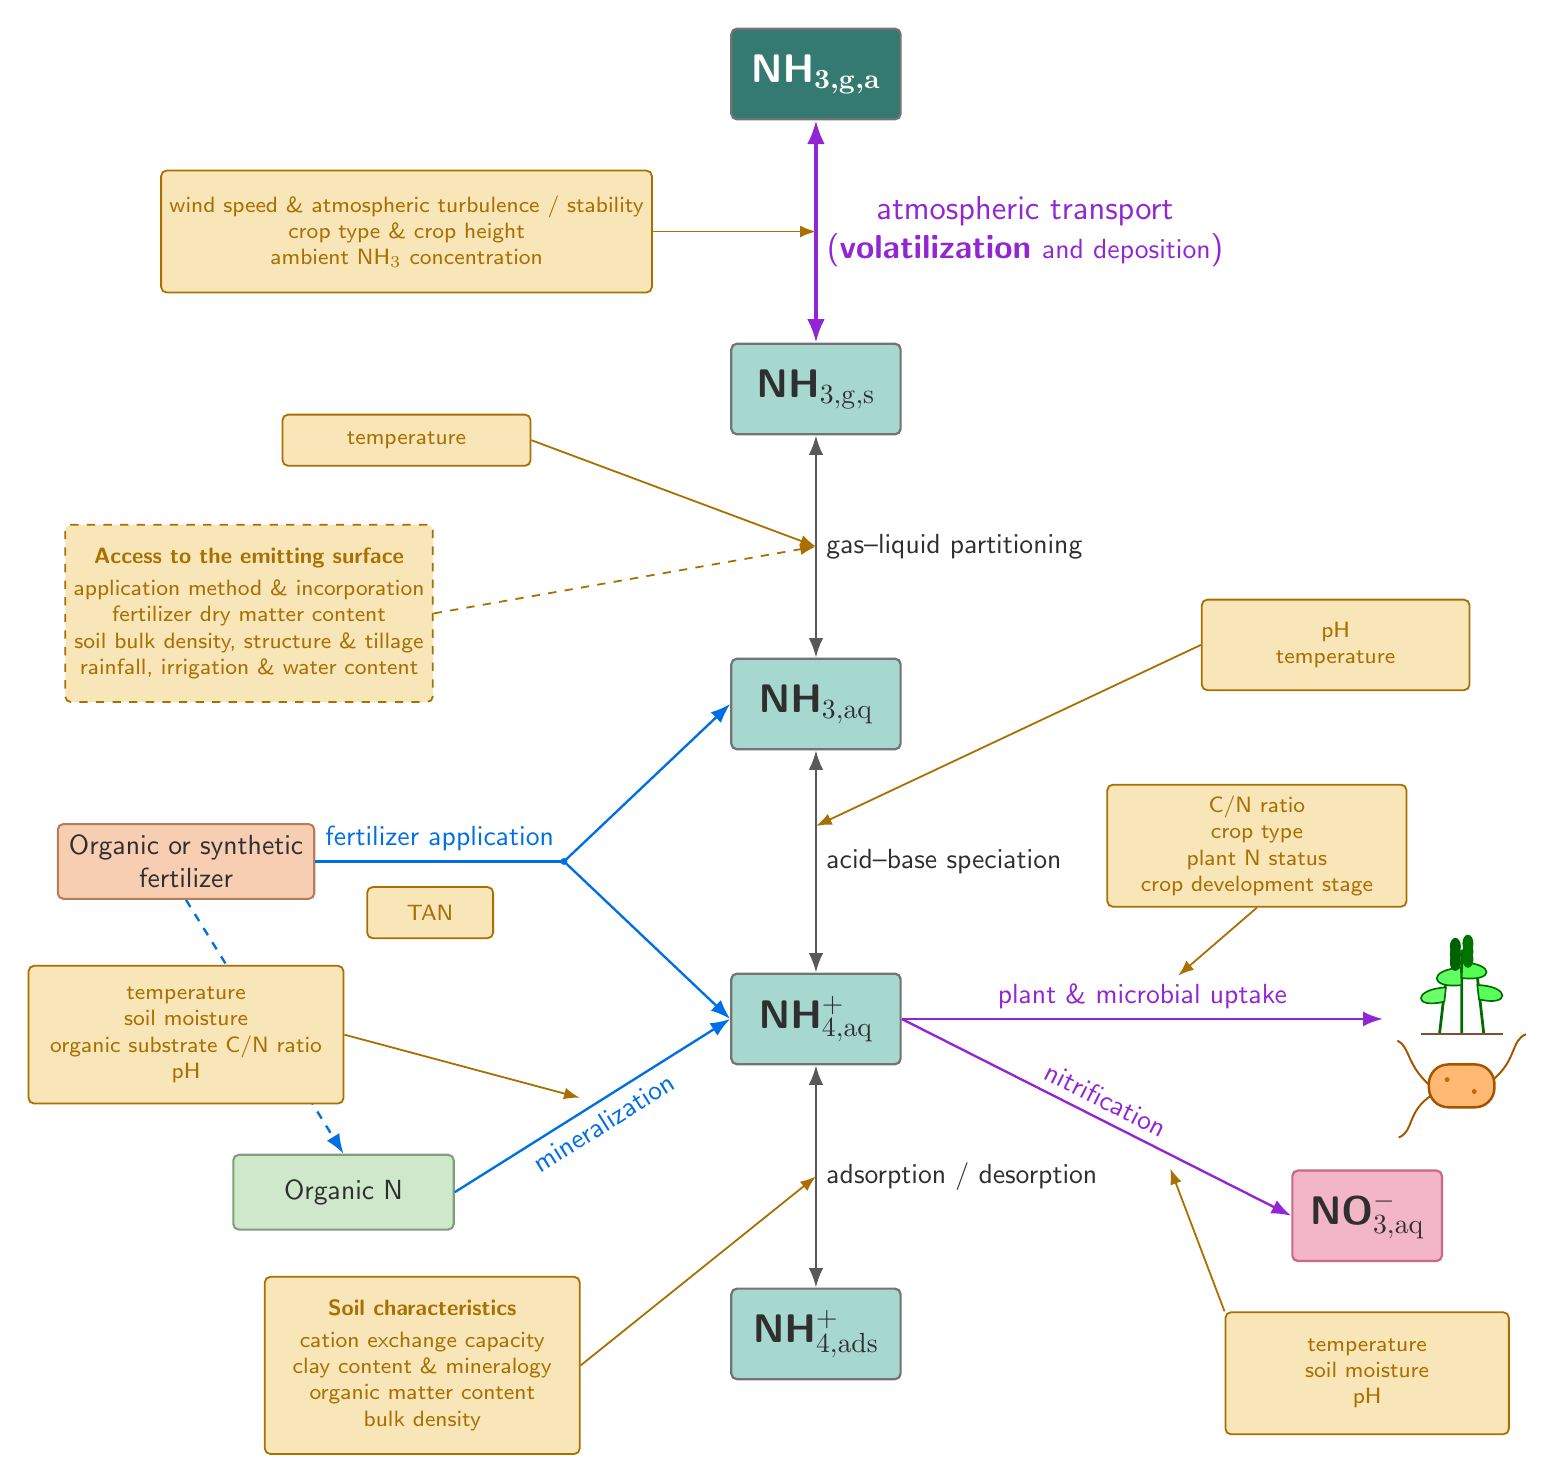
\begin{tikzpicture}[
  x=1cm,y=1cm,
  every node/.style={font=\sffamily, text=textgray},
  species/.style={
    rounded corners=2pt,
    draw=black!55,
    fill=processblue,
    line width=0.8pt,
    minimum width=2.15cm,
    minimum height=1.15cm,
    align=center,
    font=\sffamily\bfseries\Large
  },
  input/.style={
    rounded corners=2pt,
    draw=#1!75!black,
    fill=#1!55,
    line width=0.75pt,
    minimum width=2.8cm,
    minimum height=0.95cm,
    align=center,
    inner sep=4pt,
    font=\sffamily\normalsize
  },
  factor/.style={
    rounded corners=2pt,
    draw=factorochre,
    fill=factorfill!60,
    line width=0.65pt,
    minimum width=3.15cm,
    minimum height=0.65cm,
    align=center,
    inner sep=3pt,
    font=\sffamily\footnotesize,
    text=factorochre
  },
  indirectfactor/.style={
    factor,
    dashed,
    minimum width=4.3cm,
    minimum height=2.25cm
  },
  equilibrium/.style={Latex-Latex, line width=0.9pt, draw=black!65},
  flux/.style={{Latex[length=3mm]}-{Latex[length=3mm]}, line width=1.2pt, draw=outputpurple},
  inputarrow/.style={-{Latex[length=2.5mm]}, line width=0.85pt, draw=inputblue},
  outputarrow/.style={-{Latex[length=2.5mm]}, line width=0.85pt, draw=outputpurple},
  factorarrow/.style={-{Latex[length=2mm]}, line width=0.65pt, draw=factorochre},
  indirectfactorarrow/.style={factorarrow, dashed}
]

% Volatilization pathway, from the soil reservoir to the atmosphere
\node[species] (ads) at (0,-8) {NH$_{4,\mathrm{ads}}^+$};
\node[species] (nhfour) at (0,-4) {NH$_{4,\mathrm{aq}}^+$};
\node[species] (nhaq) at (0,0) {NH$_{3,\mathrm{aq}}$};
\node[species] (nhgas) at (0,4) {NH$_{3,\mathrm{g,s}}$};
\node[
  species,
  fill=atmosgreen,
  text=white,
  font=\sffamily\bfseries\Large\boldmath
] (nhair) at (0,8) {NH$_{3,\mathrm{g,a}}$};

\draw[equilibrium] (ads) --
  node[right, font=\sffamily\normalsize, align=left] {adsorption / desorption}
  (nhfour);
\draw[equilibrium] (nhfour) --
  node[right, font=\sffamily\normalsize, align=left] {acid--base speciation}
  (nhaq);
\draw[equilibrium] (nhaq) --
  node[right, font=\sffamily\normalsize, align=left] {gas--liquid partitioning}
  (nhgas);
\draw[flux] (nhgas) --
  node[right, font=\sffamily\large, align=center, text=outputpurple]
  {atmospheric transport\\(\textbf{volatilization} {\normalsize and deposition})}
  (nhair);

% Inputs to the aqueous ammoniacal nitrogen pool
\node[input=fertpastel] (fertilizer) at (-8,-2) {Organic or synthetic\\fertilizer};
\coordinate (fertsplit) at (-3.2,-2);
\draw[line width=0.85pt, draw=inputblue] (fertilizer.east) --
  node[above, font=\sffamily\normalsize, text=inputblue] {fertilizer application}
  (fertsplit);
\fill[inputblue] (fertsplit) circle (1.25pt);
\draw[inputarrow] (fertsplit) -- (nhaq.west);
\draw[inputarrow] (fertsplit) -- (nhfour.west);
\node[factor, minimum width=1.6cm] at (-4.9,-2.65) {TAN};

\node[input=organicpastel] (organicn) at (-6,-6.2) {Organic N};
\draw[inputarrow] (organicn.east) --
  node[below, sloped, font=\sffamily\normalsize, text=inputblue] {mineralization}
  (nhfour.west);

% Outputs from the aqueous ammonium pool
\node[species, minimum width=1.9cm, fill=nitratepink, draw=nitrateborder]
  (nitrate) at (7,-6.5) {NO$_{3,\mathrm{aq}}^-$};
\draw[outputarrow] (nhfour.east) --
  node[above, sloped, font=\sffamily\normalsize, text=outputpurple] {nitrification}
  (nitrate.west);

% Combined plant and microorganism uptake
\coordinate (uptakeprocess) at (4.6,-3.45);
\coordinate (uptaketarget) at (7.2,-4);
\begin{scope}[shift={(8.2,-3.7)}]
  % Stylized cereal crop
  \draw[line width=1.0pt, draw=green!42!black]
    (-0.28,-0.48) -- (-0.20,0.20)
    (0,-0.48) -- (0,0.58)
    (0.28,-0.48) -- (0.20,0.23);
  \path[draw=green!42!black, fill=green!58, line width=0.6pt]
    (-0.22,-0.08) .. controls (-0.62,-0.18) and (-0.62,0.08) .. (-0.20,0.10)
    -- cycle;
  \path[draw=green!42!black, fill=green!65, line width=0.6pt]
    (0.22,-0.05) .. controls (0.62,-0.15) and (0.62,0.12) .. (0.20,0.13)
    -- cycle;
  \path[draw=green!42!black, fill=green!62, line width=0.6pt]
    (0,0.13) .. controls (-0.42,0.08) and (-0.42,0.33) .. (-0.01,0.35)
    -- cycle;
  \path[draw=green!42!black, fill=green!68, line width=0.6pt]
    (0,0.22) .. controls (0.42,0.17) and (0.42,0.40) .. (0.01,0.42)
    -- cycle;
  \foreach \y in {0.42,0.52,0.62} {
    \fill[green!38!black] (-0.08,\y) ellipse [x radius=0.07, y radius=0.11];
    \fill[green!45!black] (0.08,\y+0.04) ellipse [x radius=0.07, y radius=0.11];
  }
  \draw[line width=0.8pt, draw=brown!65!black] (-0.52,-0.49) -- (0.52,-0.49);
\end{scope}
\draw[outputarrow] (nhfour.east) --
  node[above, font=\sffamily\normalsize, text=outputpurple] {plant \& microbial uptake}
  (uptaketarget);

\begin{scope}[shift={(8.2,-4.85)}, scale=0.8]
  \draw[line width=0.7pt, draw=orange!65!black]
    (-0.52,0.02) .. controls (-0.88,0.35) and (-0.82,0.62) .. (-1.02,0.72);
  \draw[line width=0.7pt, draw=orange!65!black]
    (-0.48,-0.15) .. controls (-0.88,-0.42) and (-0.75,-0.72) .. (-1.00,-0.82);
  \draw[line width=0.7pt, draw=orange!65!black]
    (0.50,0.10) .. controls (0.88,0.42) and (0.78,0.72) .. (1.02,0.82);
  \path[draw=orange!65!black, fill=orange!55, line width=0.9pt, rounded corners=7pt]
    (-0.52,-0.34) rectangle (0.52,0.34);
  \fill[orange!80!black] (-0.23,0.10) circle (1.1pt);
  \fill[orange!80!black] (0.20,-0.09) circle (1.1pt);
\end{scope}

% Factors controlling atmospheric transport
\coordinate (transport) at (0,6);
\node[factor, minimum width=4.2cm, minimum height=1.55cm]
  (atmosphericfactor) at (-5.2,6.0) {
  wind speed \& atmospheric turbulence / stability\\
  crop type \& crop height\\
  ambient NH$_3$ concentration
};
\draw[factorarrow] (atmosphericfactor.east) -- (transport);

% Direct and indirect controls of gas--liquid partitioning at the emitting surface
\coordinate (partition) at (0,2);
\node[factor] (temperaturefactor) at (-5.2,3.35)
  {temperature};
\draw[factorarrow] (temperaturefactor.east) -- (partition);

\node[indirectfactor] (surfaceaccess) at (-7.2,1.15) {
  \textbf{Access to the emitting surface}\\[2pt]
  application method \& incorporation\\
  fertilizer dry matter content\\
  soil bulk density, structure \& tillage\\
  rainfall, irrigation \& water content
};
\draw[indirectfactorarrow] (surfaceaccess.east) -- (partition);

% Direct controls of aqueous acid--base speciation
\coordinate (acidbase) at (0,-1.55);
\node[factor, minimum width=3.4cm, minimum height=1.15cm]
  (acidbasefactor) at (6.6,0.75) {
  pH\\
  temperature
};
\draw[factorarrow] (acidbasefactor.west) -- (acidbase);

% Main soil controls of ammonium adsorption and desorption
\coordinate (adsorption) at (0,-6);
\node[factor, minimum width=4.0cm, minimum height=2.25cm] (soilfactor) at (-5.0,-8.4) {
  \textbf{Soil characteristics}\\[2pt]
  cation exchange capacity\\
  clay content \& mineralogy\\
  organic matter content\\
  bulk density
};
\draw[factorarrow] (soilfactor.east) -- (adsorption);

% Main environmental controls of organic nitrogen mineralization
\coordinate (mineralizationprocess) at (-3.0,-5);
\node[factor, minimum width=4.0cm, minimum height=1.75cm]
  (mineralizationfactor) at (-8.0,-4.2) {
  temperature\\
  soil moisture\\
  organic substrate C/N ratio\\
  pH
};
\draw[factorarrow] (mineralizationfactor.east) -- (mineralizationprocess);

% Main controls of plant and microbial ammonium uptake
\node[factor, minimum width=3.8cm, minimum height=1.55cm]
  (uptakefactor) at (5.6,-1.8) {
  C/N ratio\\
  crop type\\
  plant N status\\
  crop development stage
};
\draw[factorarrow] (uptakefactor.south) -- (uptakeprocess);

% Main environmental controls of nitrification
\coordinate (nitrificationprocess) at (4.5,-5.9);
\node[factor, minimum width=3.6cm, minimum height=1.55cm]
  (nitrificationfactor) at (7,-8.5) {
  temperature\\
  soil moisture\\
  pH
};
\draw[factorarrow] (nitrificationfactor.north west) -- (nitrificationprocess);

% Fertilizer organic-N input, behind the foreground boxes and arrows.
\begin{scope}[on background layer]
  \draw[inputarrow, dashed] (fertilizer.south) -- (organicn.north);
\end{scope}

\end{tikzpicture}
\end{document}
